\documentclass[12pt,a4paper,portrait]{article}

\usepackage[portuguese]{babel} 	% hifenização
\usepackage[utf8]{inputenc} 	% acentos e cedilhas
\usepackage[T1]{fontenc} 		% evitar problemas com fonts
\usepackage{graphicx}
\usepackage{fancyhdr}
\usepackage{lastpage}
\usepackage[dvipsnames]{xcolor}
\usepackage{colortbl}
\usepackage{enumerate}			% Include the enumerate-package
\usepackage{listings}           % Include the listings-package
\usepackage{color}				% Include the color-package
\usepackage{siunitx}
\usepackage{textcomp}


\pagestyle{fancy}
\fancyhf{}
\rhead{Engenharia Informática 3º Ano}
\lhead{ISMAT}
\rfoot{Página \thepage \hspace{1pt} de \pageref{LastPage}}

\setcounter{secnumdepth}{5}	% actualiza o contador máximo de níveis para subsections
\setcounter{tocdepth}{5}	% actualiza o contador máximo de níveis na Tabela de Conteudo


\begin{document}
	\begin{titlepage}
	\begin{center}
	
		% Upper part of the page. The '~' is needed because \\
		% only works if a paragraph has started.
		%\includegraphics[width=0.95\textwidth]{./logo}~\\[1,5cm]
		
\includegraphics[scale=1.5]{./img/logotipo.png}
		% \includegraphics{logo_ismat}
		
		
		%\textsc{\LARGE Instituto Superior Manuel Teixeira Gomes }\\[1.5cm]
		
		\textsc{\Large Sistemas Embebidos}\\[1.5cm]
		
		% Title
		\newcommand{\HRule}{\rule{\linewidth}{0.5mm}}
		\HRule \\[0.4cm]
		{ \huge \bfseries Mini Weather Station Rev.1 \\[0.4cm] }
		
		\HRule \\[1.5cm]
		
		% discente e docente
		\noindent
		
		\begin{minipage}[t]{0.4\textwidth}
			\begin{flushleft} \large
				\emph{Discente(s):}\\
				Pedro \textsc{Roldan}\\
				Márcio \textsc{Silva}
			\end{flushleft}
		\end{minipage}%
		\begin{minipage}[t]{0.4\textwidth}
			\begin{flushright} \large
				\emph{Docente:} \\
				Mestre Melo \textsc{Pereira}
			\end{flushright}
		\end{minipage}
		
		\vfill
		
		% Bottom of the page
		{\large \today}
	
	\end{center}
\end{titlepage}
	\tableofcontents
	
	\lstdefinestyle{customc}{
	  belowcaptionskip=1\baselineskip,
	  breaklines=true,
	  frame=L,
	  xleftmargin=\parindent,
	  language=C,
	  showstringspaces=false,
	  basicstyle=\footnotesize\ttfamily,
	  keywordstyle=\bfseries\color{green!40!black},
	  commentstyle=\itshape\color{purple!40!black},
	  identifierstyle=\color{blue},
	  stringstyle=\color{orange},
      tabsize=1,
	}
	
	\newpage
	\section{Introdução}
		Uma estação meteorológica é por definição um conjunto de dispositivos que atuam no ambiente de forma a registarem diversos valores possáveis(precipitação, temperatura, humildade, luminosidade etc) e que permite a sua visualização registo e interpretação por especialistas na área da meteorologia .\\
		A previsão metateológica é na sua gênese o ato da correta interpretação de todos os valores disponíveis de forma a que seja possível uma previsão meteorológica fidedigna possível.
		\subsection{Especificações}
			A estação meteorologia Rev.1, sendo ainda um protótipo é composta pelos seguintes componentes (Arduino Uno Rev.3.0, DHT22, LDR, FC-37, SSD1306) sendo o protótipo com energia derivada do USB. \\
			\subsection{Detalhes sobre Mini Weather Station Rev.1}
			\begin{center}
				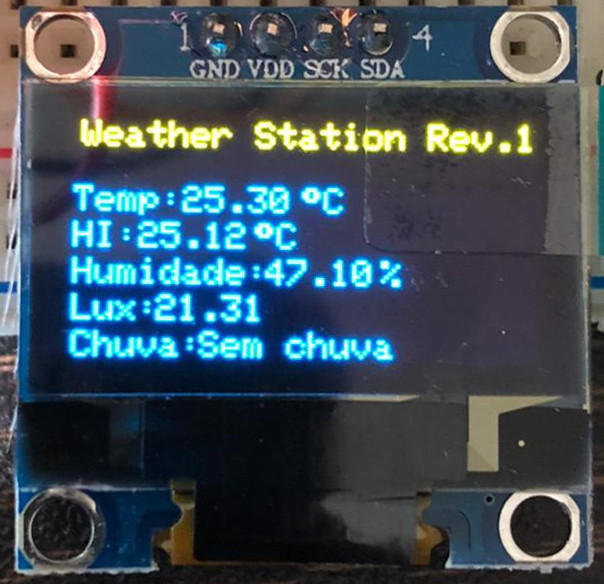
\includegraphics[scale=0.3]{./img/display_info.jpeg}
			\end{center}
			A estação meteorologia Rev.1 através dos seus sensores regista:
			\begin{itemize}
				\item Temperatura em Graus Celsius
				\item Índice de Calor em Graus Celsius
				\item Umidade em percentagem
				\item Precipitação
				\item Luminosidade em Lux
			\end{itemize}
		Como pontos em destaque temos o índice de calor que visa determinar o efeito da umidade relativa sobre a temperatura aparente do ar. Entre outras palavras é uma medida para definir a intensidade do calor que uma pessoa sente, variando em função da temperatura e umidade do ar, é calculada através da formula:\\
		\begin{center}
			
\includegraphics[scale=0.9]{./img/hi.png}
		\end{center}
		A Luminosidade expressa em Lux corresponde a densidade da intensidade luminosa, corresponde a incidência perpendicular de um lumen em uma superfície de 1m quadrado e é expressa pela formula calculada de:\\\\
		Valor do Lux = (250.000000/(0.0048828125 * Ldr))- 50.000000;\\
		
	
	
			\subsubsection{Se02.ino}
			Ficheiro com a programação necessária a ser enviado para a plataforma arduino Rev.3\\
			
			Definição de pins e instanciação de dispositivos 
				\lstset{escapechar=@,style=customc}
				\begin{lstlisting}
				#define DHTPIN 2          //pin DHT sensor 
				#define DHTTYPE DHT22     //tipo de sensor
				#define OLED_ADDR   0x3C  // endereço i2c oled
				#define LDRPIN A0         //pin DHT sensor
				#define FC37PINA A2       //pin FC37 analogico sensor
				#define FC37PIND 7        //pin FC37 digital sensor 
				
				DHT dht(DHTPIN, DHTTYPE); //instacia sensor
				
				// reset pin not used on 4-pin OLED module
				Adafruit_SSD1306 display(-1);  // -1 = no reset pin
				\end{lstlisting}
				\newpage
				De seguida são iniciadas as variáveis de controlo
				\lstset{escapechar=@,style=customc}
				\begin{lstlisting}
				float humidityValue = 0;      // humidade
				float temperatureValue = 0;   // temperatura
				float heatIndexValue = 0;     // heat index
				float lightValue = 0;         // light value
				float luxValue = 0;           // lux value
				float adcValue =0.0048828125;
				int rainMax = 1024;           // rain max value
				int rainMin = 0;              // rain min value
				int rainValue = 0;            // rain value
				int rainMap = 0;              // rain converted map values
				String rainDescription;       // rain description
				
				\end{lstlisting}
				É efetuado o setup de dispositivos e pins
				\lstset{escapechar=@,style=customc}
				\begin{lstlisting}
				display.begin(SSD1306_SWITCHCAPVCC, OLED_ADDR);
				pinMode(FC37PIND, INPUT);
				dht.begin();
				\end{lstlisting}
				Leitura dos diversos sensores com ciclo de 2s entre medições
				\lstset{escapechar=@,style=customc}
				\begin{lstlisting}
				humidityValue = dht.readHumidity(); // valor humidade em celcius
				temperatureValue = dht.readTemperature(); // valor temperatura celcius 
				lightValue = analogRead(LDRPIN);
				rainValue = analogRead(FC37PINA);
				\end{lstlisting}
				Calculo de luminosidade em Lux
				\lstset{escapechar=@,style=customc}
				\begin{lstlisting}
				  luxValue = (250.000000/(adcValue * lightValue))- 50.000000; // formula p conversao para lux
				\end{lstlisting}
				Calculo do índice de calor em Graus Celsius
				\lstset{escapechar=@,style=customc}
				\begin{lstlisting}
				heatIndexValue = dht.computeHeatIndex(temperatureValue, humidityValue, false);
				\end{lstlisting}
			\subsubsection{Esquema}
				\begin{center}
				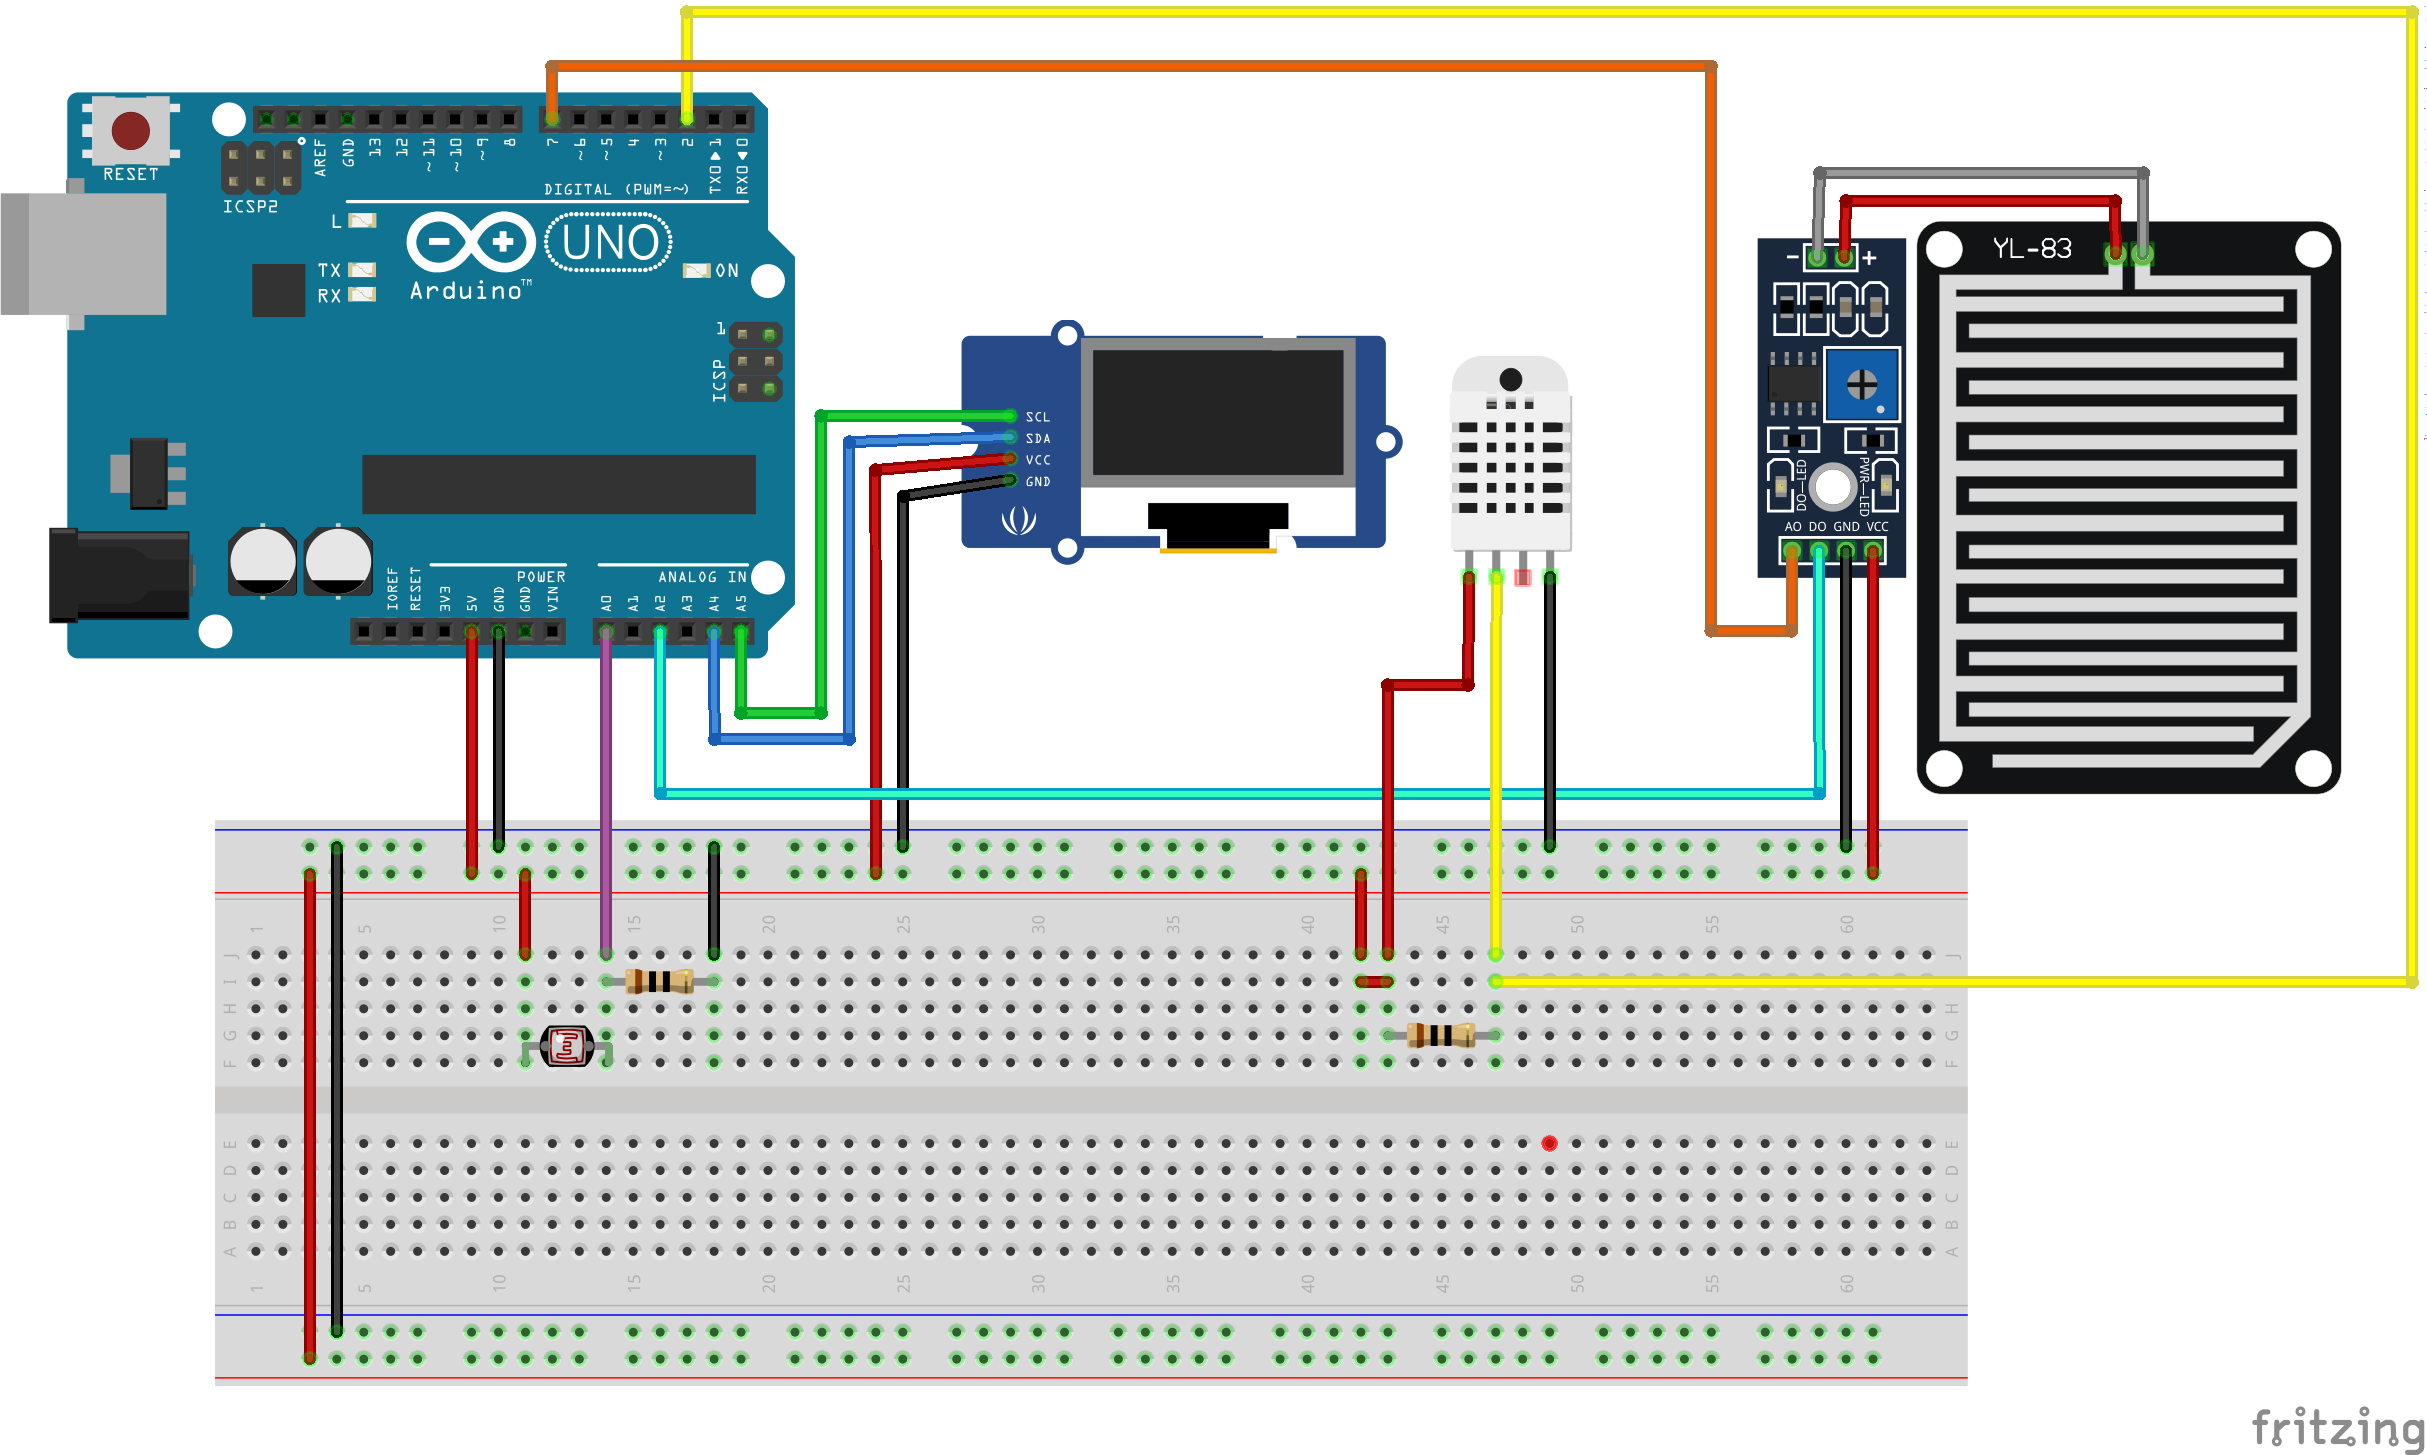
\includegraphics[scale=0.6]{./img/view.png}
				Protótipo\\
			\end{center}
			\begin{center}
				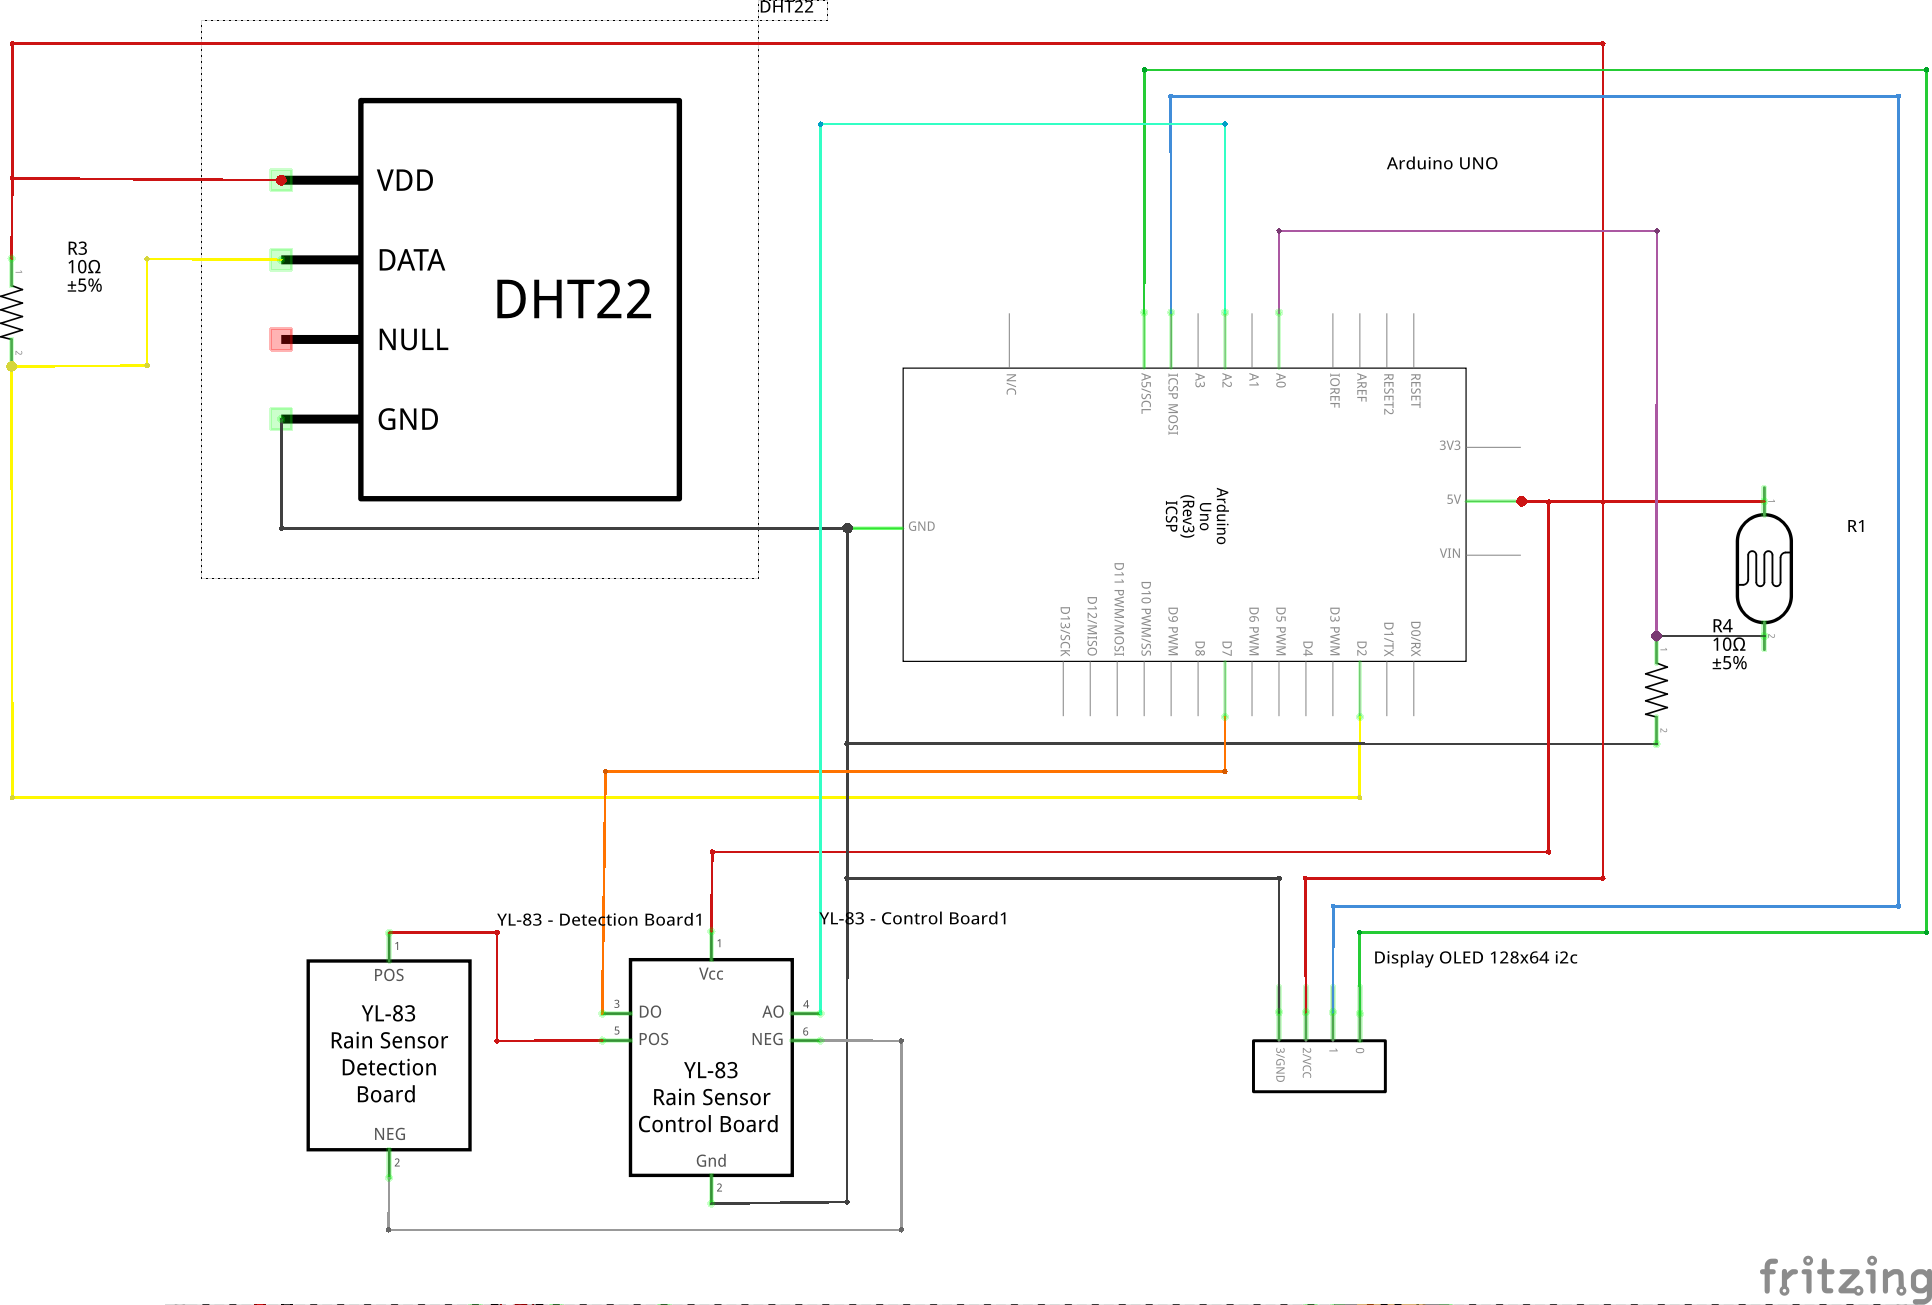
\includegraphics[scale=0.75]{./img/esquema.png}
				Sistema Digital\\	
			\end{center}
			

		\subsection{Componentes}		
			\subsubsection{Arduino UNO Rev.3}
				\begin{center}
					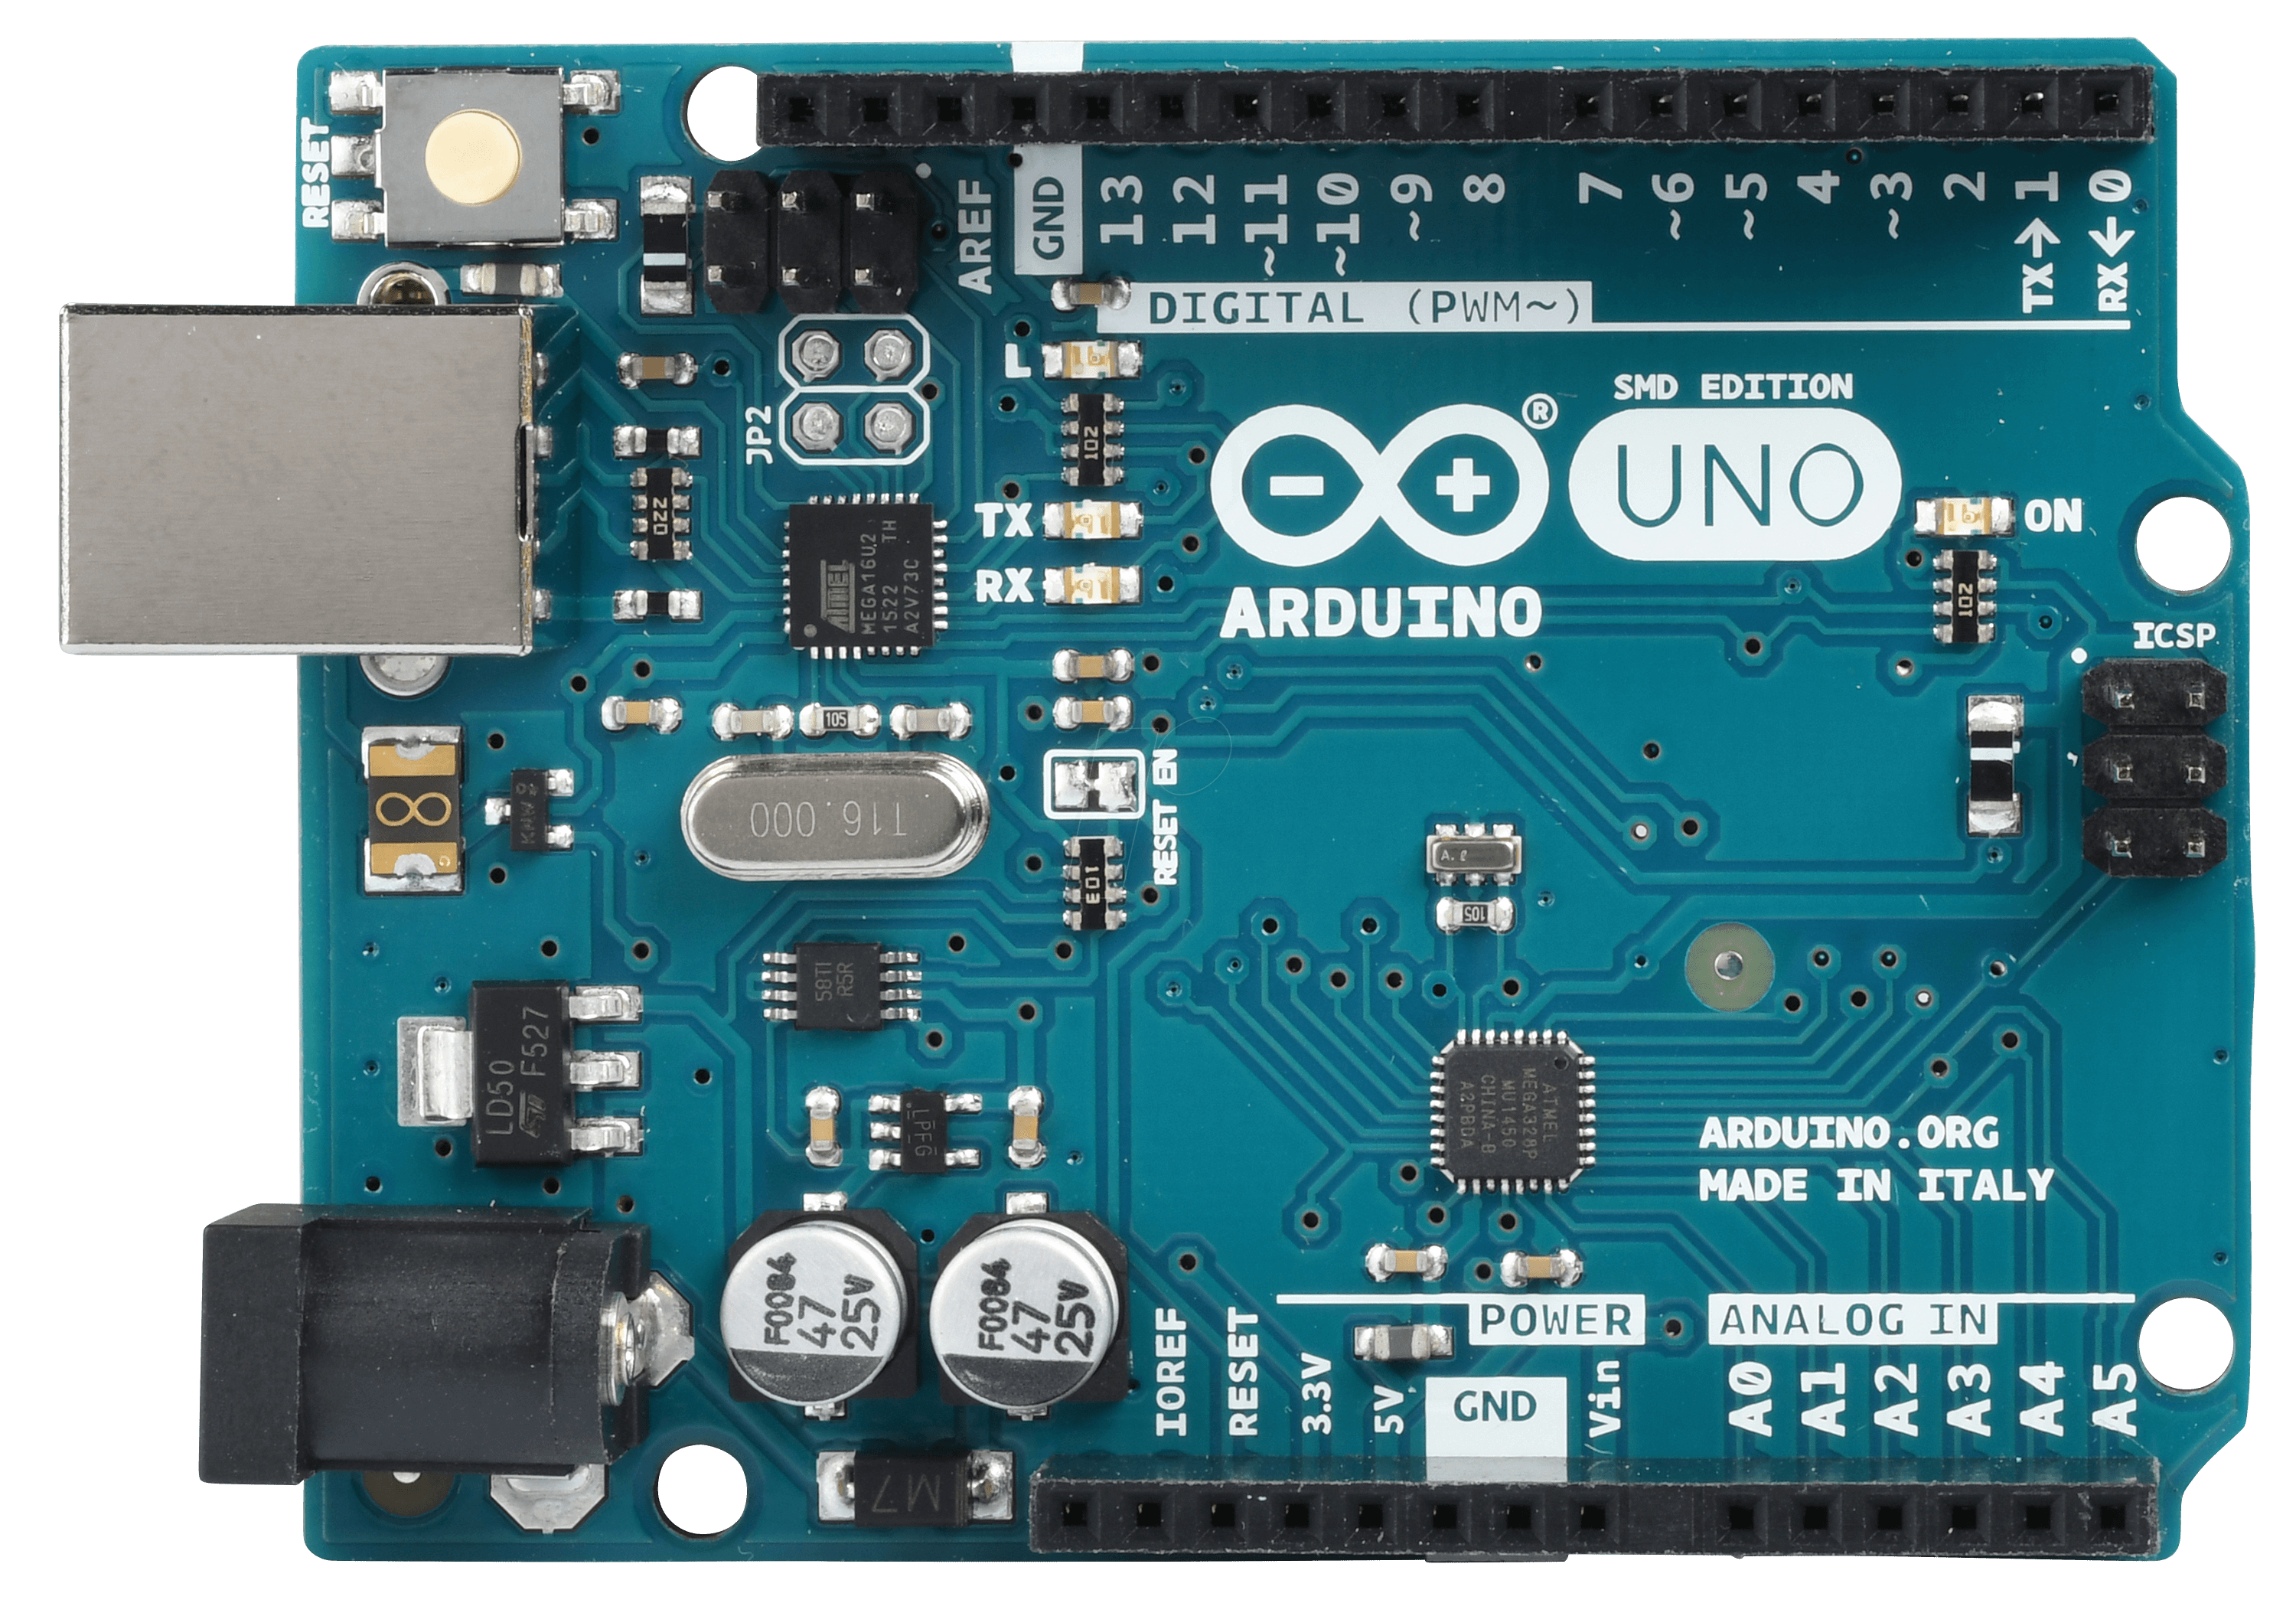
\includegraphics[scale=0.07]{./img/arduino_uno.png}
				\end{center}
			\cite{arduinoCompany}
			\begin{itemize}
				\item Microcontroller: ATmega328P
				\item Operating Voltage: 5V
				\item Input Voltage (recommended): 7-12V
				\item Input Voltage (limit): 6-20V
				\item Digital I/O Pins: 14 (of which 6 provide PWM output)
				\item PWM Digital I/O Pins: 6
				\item Analog Input Pins: 6
				\item DC Current per I/O Pin: 20 mA
				\item DC Current for 3.3V Pin: 50 mA
				\item Flash Memory: 32 KB (ATmega328P) of which 0.5 KB used by bootloader
				\item SRAM: 2 KB (ATmega328P)
				\item EEPROM: 1 KB (ATmega328P)
				\item Clock Speed: 16 MHz
				\item LED\textunderscore BUILTIN: 13
				\item Length: 68.6 mm
				\item Width: 53.4 mm
				\item Weight: 25 g
			\end{itemize}
			\subsubsection{DHT22}
				\begin{center}
					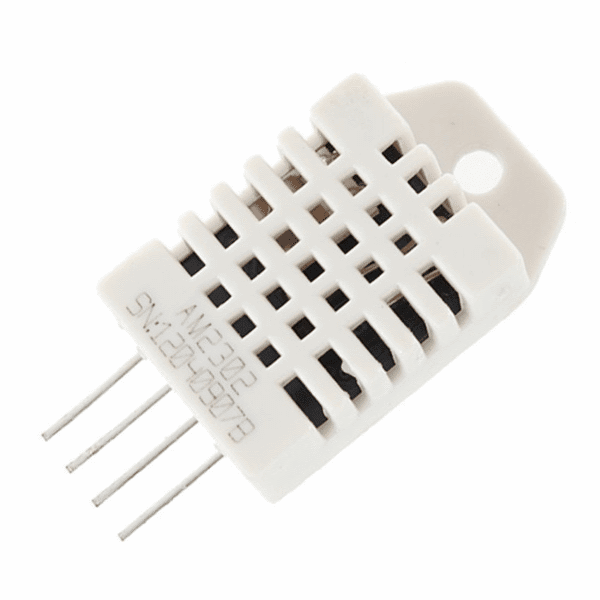
\includegraphics[scale=0.2]{./img/dht22.png}
				\end{center}
			\begin{itemize}
				\item Operating Voltage: 3.5V to 5.5V
				\item Operating current: 0.3mA (measuring) 60uA (standby)
				\item Output: Serial data
				\item Temperature Range: -40\textdegree C to 80\textdegree C
				\item Humidity Range: 0\% to 100\%
				\item Resolution: Temperature and Humidity both are 16-bit
				\item Accuracy: +/-0.5°C and +/-1\%
			\end{itemize}
			\subsubsection{Ldr}
				\begin{center}
					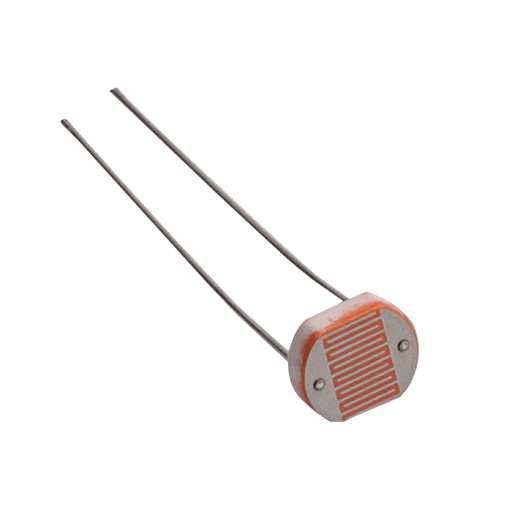
\includegraphics[scale=0.3]{./img/ldr.png}
				\end{center}
			\begin{itemize}
				\item Can be used to sense Light
				\item Easy to use on Breadboard or Perf Board
				\item Easy to use with Microcontrollers or even with normal Digital/Analog IC
				\item Small, cheap and easily available
				\item Available in PG5 ,PG5-MP, PG12, PG12-MP, PG20 and PG20-MP series
			\end{itemize}
			\subsubsection{FC-37}
				\begin{center}
					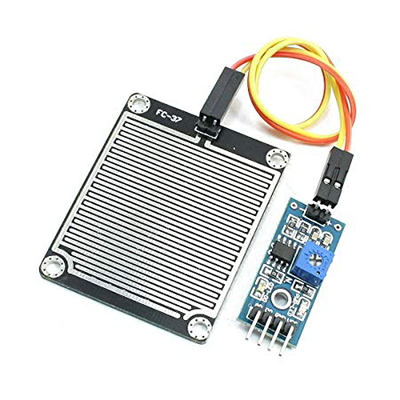
\includegraphics[scale=0.5]{./img/fc-37.png}
				\end{center}
			\begin{itemize}
				\item Adopts high quality of RF-04 double sided material
				\item Area: 5cm x 4cm nickel plate on side,
				\item Anti-oxidation, anti-conductivity, with long use time;
				\item Comparator output signal clean waveform is good, driving ability, over 15mA;
				\item Potentiometer adjust the sensitivity;
				\item Working voltage 5V;
				\item Output format: Digital switching output (0 and 1) and analog voltage output AO;
				\item With bolt holes for easy installation;
				\item Small board PCB size: 3.2cm x 1.4cm;
				\item Uses a wide voltage LM393 comparator
			\end{itemize}
			\subsubsection{OLED SSD1306}
				\begin{center}
					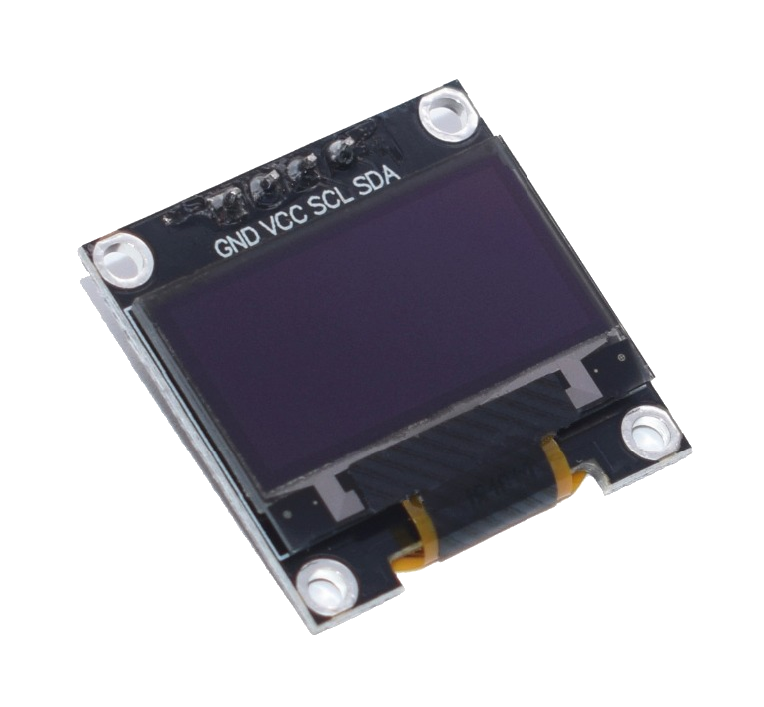
\includegraphics[scale=0.6]{./img/display_oled.png}
				\end{center}
			\begin{itemize}
				\item Resolution: 128 x 64 dot matrix panel 
				\item Power supply 
				\begin{itemize}
					\item VDD = 1.65V to 3.3V for IC logic
					\item VCC = 7V to 15V for Panel driving 
				\end{itemize}
				\item For matrix display
				\begin{itemize}
					\item OLED driving output voltage, 15V maximum 
					\item Segment maximum source current: 100uA 
					\item Common maximum sink current: 15mA 
					\item 256 step contrast brightness current control 
				\end{itemize}
				\item Embedded 128 x 64 bit SRAM display buffer 
				\item Pin selectable MCU Interfaces: 
				\begin{itemize}
					\item 8-bit 6800/8080-series parallel interface 
					\item 3 /4 wire Serial Peripheral Interface 
					\item I2C Interface  
				\end{itemize}
				\item Screen saving continuous scrolling function in both horizontal and vertical direction 
				\item RAM write synchronization signal 
				\item Programmable Frame Rate and Multiplexing Ratio 
				\item Row Re-mapping and Column Re-mapping 
				\item On-Chip Oscillator 
				\item Chip layout for COG \& COF 
				\item Wide range of operating temperature: -40\textdegree C to 85\textdegree C
			\end{itemize}
			\newpage
		\subsection{Bibliotecas}
			\subsubsection{DHT.h}
			Biblioteca que permite interconectividade entre os sensores da gama DHT(11, 22, etc).\\\\
			https://github.com/adafruit/DHT-sensor-library\\
			\cite{adafruitdht}
			\subsubsection{Wire.h}
			Biblioteca que permite comunicação com dispositivos I2C/TWI.\\
			Uno I2C/TWI pins A4(SDA), A5(SCL).\\\\
			https://github.com/esp8266/Arduino/blob/master/libraries/Wire/Wire.h\\
			\cite{wire}
			\subsubsection{Adafruit\textunderscore GFX.h}
			Biblioteca de core gráfica.\\\\
			https://github.com/adafruit/Adafruit-GFX-Library/blob/master/Adafruit \textunderscore GFX.h\\
			\cite{adafruitGFX}
			\subsubsection{Adafruit\textunderscore SSD1306.h}
			Biblioteca de interface para dispositivos SSD1306 OLED e monocromáticos de 128x64 e de 128x32.\\\\
			https://github.com/adafruit/Adafruit\textunderscore SSD1306/blob/master/Adafruit\textunderscore SSD1306.h\\
			\cite{adafruitSSD1306}
			\newpage
	\section{Enquadramento}
	O trabalho descrito neste relatório foi realizado em linguagem derivada de C na plataforma Arduino.
		\subsection{Motivação}
		A principal motivação para a realização deste trabalho, resulta da importância na resolução dos graves problemas climáticos que assombram este seculo. E demostrar conhecimentos alcançados na disciplina de Sistemas Embebidos.
		\subsection{Objetivos}
		O objetivo deste trabalho prático é a criação de uma mini estação meteorológica que permita realizar leituras através dos sensores disponibilizados, utilizando a plataforma de micro controlador arduino.
	\section{Conclusões}
	A weather station Rev.1 é uma estação meteorológica concebida para monitorizar e registar dados meteorológicos adquiridos através de diversos sensores assente numa plataforma amplamente conhecida arduino.\\
	Foi sem duvida um desafio interessante, mas que por limitação de tempo, deixa ainda uma larga margem para melhoramentos, tanto a inclusão de mais sensores para recolha de dados, sistemas de alimentação solar(painéis solares e baterias), sistemas de controlo de energia(deepsleep), estrutura física resistente em intempéries e sistemas de comunicação de longa distancia(LoRa) e envio de dados para plataformas digitais(web services).\\
	
	\newpage
	\section{Bibliografia}
	\bibliographystyle{plain}
	\bibliography{bibliotecas}
	
	\newpage
	\section{Anexos}
	Ficheiro "relatorio.pdf" e estrutura de directoria "meteo" com o ficheiro "Se\textunderscore 02.ino" compactados num ficheiro "trabalho.rar".\\\\
	Não existem quaisquer códigos ou listagens adicionais.					
\end{document}          
